\textcolor{red}{$\rightarrow$ TODO: Explanation of the PG data model chosen - details, reason why...}

\begin{comment}
\textcolor{gray}{Nowadays data are in motion, change continuously and are -possibly- unbounded implying data
sources that are also constantly evolving. From the data persistence point of view this reality breaks the
usual paradigm of having dynamic but stable data sources. This, together with the increasing number
applications based on data streams for taking critical decisions in real time, raises the need for re-thinking
both the data and the query models to fit these new requirements. Therefore, under these circumstances,
it seems reasonable that a suitable data model is a continuously evolving data graph.\\
...
Regarding the data model, the new nature of data requires a de facto new database paradigm
-continuously evolving databases- where data can be both stable and volatile. Even though
evolving databases can be implemented according to any approach, graph databases seem
especially well suited here [1, 2]. Indeed, the natural way to process evolving graphs as streams
of edges gives insights on how to proceed in order to maintain dynamic graph databases. Hence,
we consider that a suitable data model is a continuously evolving data graph, a graph having
persistent (stable) as well as non persistent (volatile) relations. Stable relations correspond
to edges occurring in standard graph databases while volatile relations are edges arriving indata streams during a set time interval. Once this time interval is over, the relations are not
longer valid so that there is no need to store them in the (stable) graph database. However,
when required -as for further legal or auditing purposes- timestamped occurrences of volatile
relations can be kept in a log file. Volatile relations induce subgraphs that exist only while the
relations are still valid. Without loss of generality, in this work we consider property graphs
(PG) [3, 4] as the basic reference data model. As an example, Figure 1a depicts part of a schema
of a PG database where stable relations correspond to the data that a bank typically gathers
on its issued cards, ATMs (Automated Teller Machines) network, etc. Volatile relations model
the interaction between cards and ATM entities}
\end{comment}

The property graph data model consists of two sub property graphs: a stable and a volatile property graph. On the one hand, the stable is composed of the static part of the data that a bank typically gathers such as information about its clients, cards, ATMs (Automated Teller Machines). 
On the other hand, the volatile property graph models the transaction operations, which defines the most frequent and reiterative kind of interaction between entities of the data model.\\
The main difference and the main reason for this separation is the semantics with which we intentionally define each of the subgraphs: the stable will be understood like a fixed static bank database, whereas the volatile will be understood as the data model to define the transactions, as continuous interactions between the entities of the model, which will not be permanently saved, but instead, only for a certain window of time under the mission of detecting anomalous bank operations. Note that we will only model the transaction interaction in the volatile subgraph, only letting them occur here.
This separation will allow us to have a really simple and light property graph schema single-centered on the transactions with the minimal needed information (mostly identifiers of the entities a transaction links) and another, the stable, acting as a traditional bank database schema, from which to obtain the information details of the entities.

\subsection{Property Graph Design}

In what follows we provide the description of the design of our proposed
Property Graph data model, divided into the stable and volatile property
graphs.

\subsubsection{Stable Property Graph}

Due to the confidential and private nature of bank data, it was
impossible to find a real bank dataset nor a real bank data model. Therefore, we devoloped our own proposal of a bank database model.
We propose a simplified data model where the defined entities, relations and properties are reduced to the essential ones.
Although it is obvious that a real bank data model is way more complex than the one we propose, we believe that ours is relevant and representative enough and therefore sufficient for the purpose of our work. 

\begin{figure}[H]
    \centering
    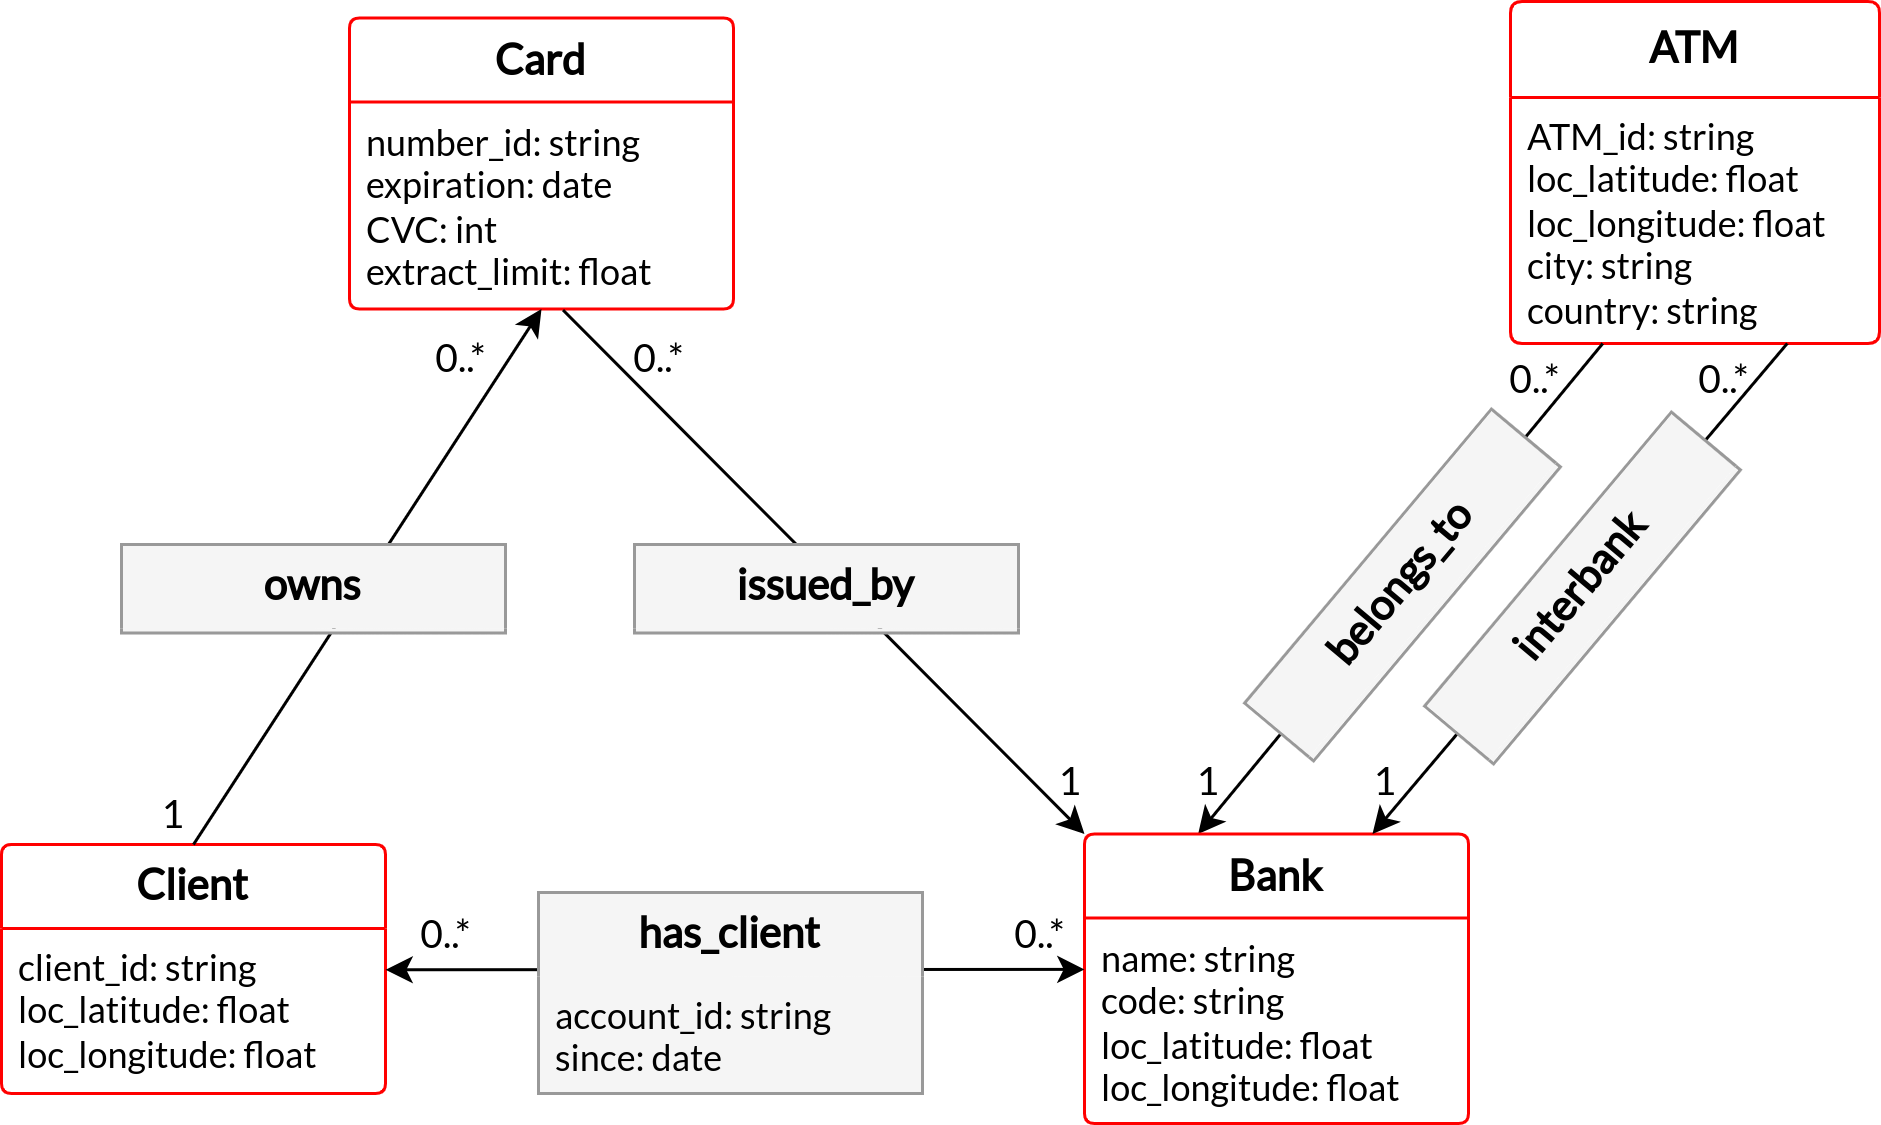
\includegraphics[scale = 0.7]{sections/1-DataModel/images/PG-stable-edit-cardinal.png}
    \caption{Initial bank stable property graph model}
    \label{img:initial-pg-stable}
\end{figure}

% TODO: Cómo pongo que se entienda bien el 1er modelo y su correspondiente transformación al segundo y definitivo: explicando también en el medio las entidades, relaciones y atributos y su elección.
A first model proposal was the one shown in Figure \ref{img:initial-pg-stable}.
Basically, the idea of this first model attempt was to capture the data that a bank system database typically gathers.
It contains four entities: Bank, ATM, Client and Card with their respective properties, and the corresponding relationships between them.
The relations are: a directed relationship from Client to Card \texttt{owns} representing that a client can own multiple credit cards and that a card is owned by a unique client, then a bidirectional relation \texttt{has\_client} between Client and Bank; representing bank accounts of the clients in the bank. The relation between Card and Bank to represent that a card is \texttt{issued\_by} the bank, and that the bank can have multiple cards issued. Finally, the relations \texttt{belongs\_to} and \texttt{interbank} between the ATM and Bank entities, representing the two different kinds of ATMs depending on their relation with the bank; those ATMs owned and operated by the bank and those that, while not owned by the bank, are still accesible for the bank customers to perform transactions.

\begin{figure}[H]
    \centering
    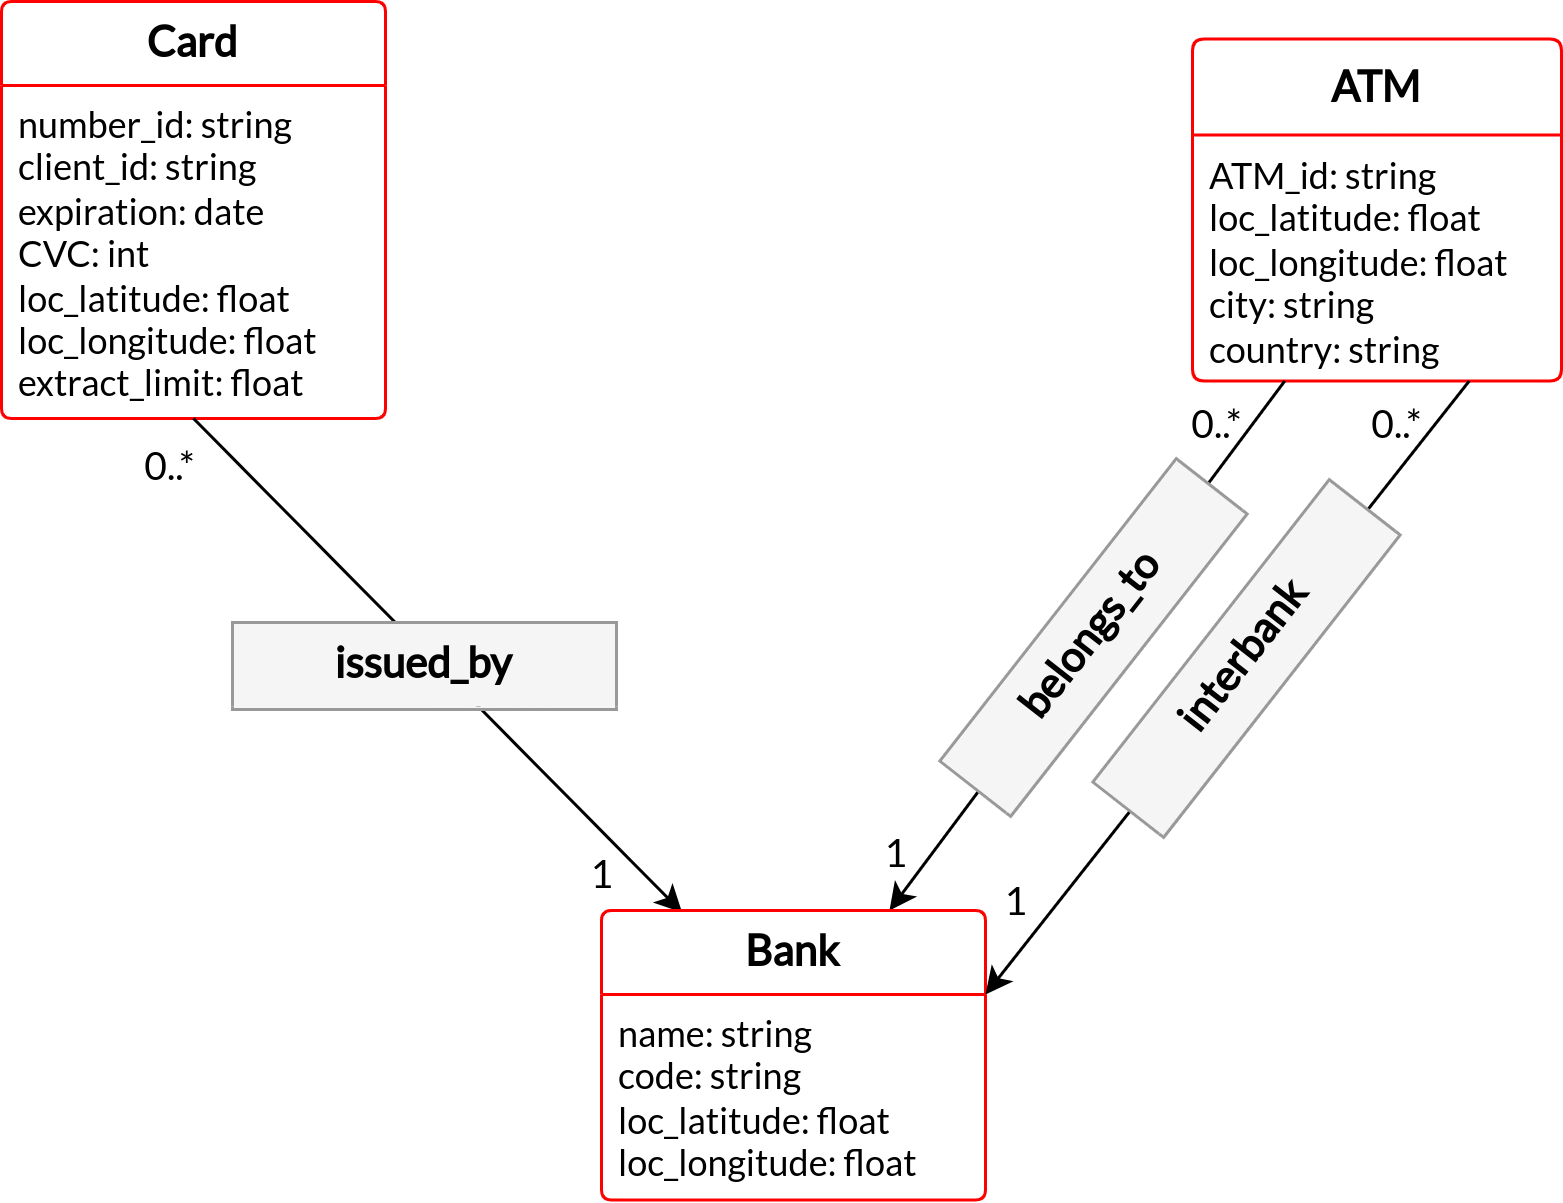
\includegraphics[scale = 0.7]{sections/1-DataModel/images/PG-stable-1-edit-cardinal.png}
    \caption{Definitive stable property graph model}
    \label{img:pg-stable-def}
\end{figure}

However, the final version of the model (see Figure \ref{img:pg-stable-def}) was simplified to reduce it to the minimal needed entities. In particular, we decided to remove the Client entity and to merge it inside the Card entity. This reduction allows to simplify the stable property graph to only three entities. 
For this, all the Client attributes were included in the Card entity. In the initial schema the Client entity was defined with three attributes: the identifier of the client and the GPS coordinates representing the usual residence of the client. This change is done while preserving the restriction of a Card belonging to a unique client the same way it was previously done with the relation between Card and Client \texttt{owns} in the initial schema, which now is therefore removed. \\
% Account relation removed
Another derived consequence of this simplification is the removal of the other relation that the Client entity had with other entities: the \texttt{has\_client} relation between Client and Bank, which was originally made with the intention of representing the bank accounts between clients and banks. Maintaining a bank account would imply having to consistently update the bank account state after each transaction of a client, complicating the model. Nevertheless, we elimintate the bank account relation, since its removal is considered negligible and at the same time helpful for the simplification of the model needed for the purposes of our work. However, for the sake of completeness the attribute \textit{extract\_limit} is introduced in the Card entity, representing a money amount limit a person can extract, which will be related with the amount of money a person owns. This will allow the detection of anomalies related with frequent or very high expenses.


\begin{comment}
The final entities and their selected attributes are described in what follows:

\paragraph{Entities\\}

\paragraph{Bank}

\begin{itemize}
\item[-] name: Bank name.
\item[-] code: Bank identifier code.
\item[-] loc\_latitude: Bank headquarters GPS-location latitude.
\item[-] loc\_longitude: Bank headquarters GPS-location longitude.
\end{itemize} 

\begin{figure}[H]
    \centering
    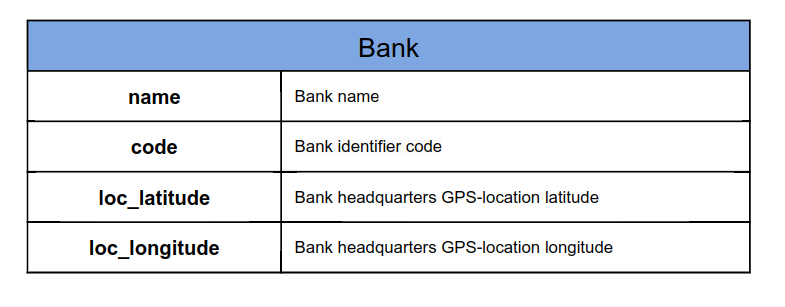
\includegraphics[scale = 0.4]{images/bank.png}
    \caption{Bank entity attributes}
    \label{img:pg-bank}
\end{figure}

\paragraph{ATM}

\begin{itemize}
\item[-] ATM\_id: Unique identifier of the ATM.
\item[-] loc\_latitude: GPS-location latitude where the ATM is located.
\item[-] loc\_longitude: GPS-location longitude where the ATM is located.
\item[-] city: City in which the ATM is located.
\item[-] country: Country in which the ATM is located.
\end{itemize}

\begin{figure}[H]
    \centering
    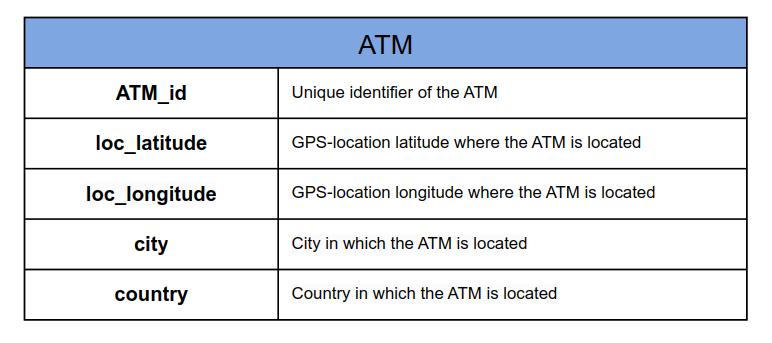
\includegraphics[scale = 0.4]{images/atm.png}
    \caption{ATM entity attributes}
    \label{img:pg-atm}
\end{figure}


\paragraph{Card}

\begin{itemize}
\item[-] number\_id: Unique identifier of the card.
\item[-] client\_id: Unique identifier of the client.
\item[-] expiration: Validity expiration date of the card.
\item[-] CVC: Card Verification Code.
\item[-] extract\_limit: Limit amount of money extraction associated with the card.
\item[-] loc\_latitude: Client address GPS-location latitude.
\item[-] loc\_longitude: Client address GPS-location longitude.
\end{itemize}

\begin{figure}[H]
    \centering
    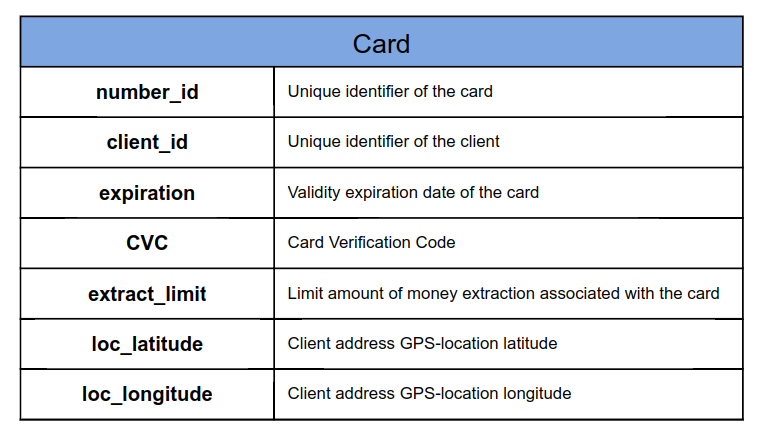
\includegraphics[scale = 0.4]{images/card.png}
    \caption{Card entity attributes}
    \label{img:pg-card}
\end{figure}

Note that for both the ATM and the Card entities we have the GPS coordinates information. In the first case referring to the geolocation of each specific ATM and in the last case referring to each specific client address geolocation. This will be useful to be able to detect transaction frauds related to geolocation distances.

Note that the client is completely anonymized in the system (no name, surname, age, or any other confidential details) by using only a client\_id. For the present purpose it is enough to uniquely identify each client.

% Relations -> and its attributes
\paragraph{Relations}
There are only two relations in the final stable subgraph, that is, the ones that are left after the deletion of the Client entity from the first version of the stable subgraph; the relation "issued\_by" between the Card and the Bank entities and the "belongs\_to" between ATM and Bank entities. For the moment they do not have any attribute, however they could potentially be added in the case this was needed.

\end{comment}

\subsubsection{Volatile property graph}
\textcolor{red}{$\rightarrow$ TODO: describe}

\begin{comment}
It contains the minimal needed information to be able to recognize the anomaly fraud patterns we want to identify.
This subgraph describes the most volatile part of our model, meaning the transactions between the client's cards and the ATMs. The idea is to have a data model to define the transactions, as continuous temporal interactions between the Card and ATM entities, restricting these kind of relations to the volatile subgraph.
The idea is to have a really simple and light property graph schema single-centered on the transactions. For that the Card and ATM entities will be simplified to the last bullet, containing only the identifier of the both entities that each transaction relation matches. These identifiers will be enough to be able to recover, if needed, the whole information about the specific Card or ATM entity in the stable subgraph.

\begin{figure}[H]
    \centering
    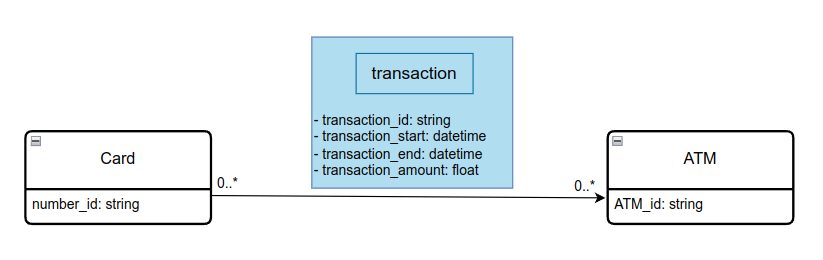
\includegraphics[scale = 0.45]{images/diagPG-volatile.png}
    \caption{Volatile property graph model}
    \label{img:pg-stable}
\end{figure}

Following this idea of volatile subgraph, the Card and ATM entities and transaction relations of it will not be permanently saved, but instead, only for a certain window of time under the mission of detecting anomalous bank operations. 

The transaction relation will include some attributes that will be essential for the detection of the fraud patterns, in particular:

\begin{itemize}
\item[-] transaction\_id: Unique identifier for each transaction in the database.
\item[-] transaction\_start: Datetime when the transaction started. Format: DD/MM/YYYY HH:MM (ex. 1/1/2022 4:50).
\item[-] transaction\_end: Datetime when the transaction was completed. Format: DD/MM/YYYY HH:MM (ex. 1/1/2022 4:54).
\item[-] transaction\_amount: Amount of money involved in the transaction.
\end{itemize}

\begin{figure}[H]
    \centering
    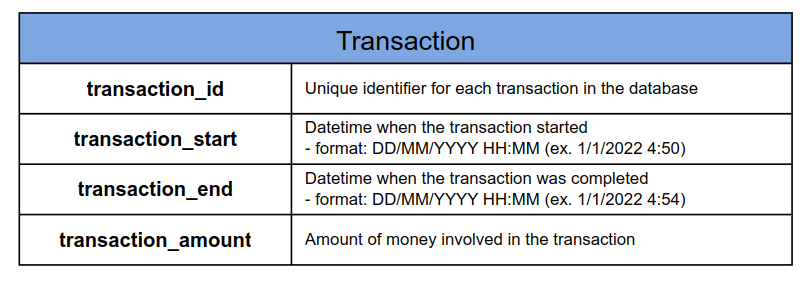
\includegraphics[scale = 0.40]{images/transaction.png}
    \caption{Transaction relation attributes}
    \label{img:pg-stable}
\end{figure}
\end{comment}
\textcolor{green}{\rule{\linewidth}{0.4mm}}
\subsection{Synthetic dataset creation}

As mentioned, given the confidential and private nature of bank data, it was not possible to find
any real bank datasets. In this regard, a synthetic property
graph bank dataset was built based on the \emph{Wisabi Bank Dataset}\footnote{\href{https://www.kaggle.com/datasets/obinnaiheanachor/wisabi-bank-dataset}{Wisabi bank dataset on kaggle}}. It is a fictional banking dataset that was made publicly available in
the Kaggle platform.

This synthetic bank dataset was considered of interest as a base for the synthetic bank
database that we wanted to develop. The interest to use this bank dataset as a base was mainly because of its size: it contains 8819 different customers, 50 different ATM locations and 2143838 transactions records of the different customers during a full year (2022). Additionally, it provides good heterogenity on the different kind of transactions: withdrawals, deposits, balance inquiries and transfers.

The main uses of this bank dataset are the obtention of a geographical distribution for
the locations of our generated ATMs and the construction of a card/client \emph{behavior},
for which the data of the \emph{Wisabi Bank Dataset} will be used.

\paragraph{Details of the \emph{Wisabi Bank Dataset}}
The \emph{Wisabi Bank Dataset} consists on ten CSV tables. Five of them are of transaction records of five different states of Nigeria (Federal Capital Territory, Lagos, Kano, Enugu and Rivers State) that refers to transactions of cardholders in ATMs. In particular they contain 2143838 transactions records done during the year 2022, of which 350251 are in Enugu, 159652 in Federal Capital Territory, 458764 in Kano, 755073 in Lagos and 420098 in Rivers. Then, the rest of the tables are: a customers table (`customers\_lookup`) where the data
of 8819 different cardholders is gathered, an ATM table (`atm\_location lookup`) with
information of each of the 50 different locations of the ATMs, and then three remaining
tables as complement of the previous ones (`calendar lookup`, `hour lookup` and 
`transaction\_type lookup`) 
(\href{https://app.diagrams.net/#G1eAn47YR7-zPNE5KgStkA6_IJcxZRYgX8#%7B%22pageId%22%3A%22R2lEEEUBdFMjLlhIrx00%22%7D}{tables summary}).

In what follows we give the details on the generation of the instances of our static database
entities.
For simplicity and to do it in a more stepwise manner, we are going to first create all the CSV data tablesfor the nodes and for the relations in the corresponding format and then we will populate the Neo4j GDB with them.

$\rightarrow$ To do the generation of a stable bank database use the Python program \texttt{bankDataGenerator.py}, in which you will have to enter the bank properties' values, 
as well as the parameters on the number of the bank ATMs and Cards: \texttt{n} and \texttt{m}, respectively.

\subsubsection*{Bank}

Since a unique bank instance is considered, the values of the properties of the bank node are 
manually assigned, leaving them completely customisable. Bank node type properties consist
on the bank \emph{name}, its identifier \emph{code} and the location
of the bank headquarters, expressed in terms of \emph{latitude} and \emph{longitude}
coordinates, as seen in Table \ref{table:bank-node-properties}.
For the bank, we will generate \texttt{n} ATM and \texttt{m} Card entities. Note that 
apart from the generation of the ATM and Card node types we will also need to generate 
the relationships between the ATM and Bank entities (\texttt{belongs\_to} and \texttt{interbank}) 
and the Card and Bank entities (\texttt{issued\_by}).

\begin{table}[H]
    \centering
      \begin{tabular}{|l|l|}
      \hline
      \textbf{Name}        & \textbf{Description and value}                                      \\ \hline
      \texttt{name}         & Bank name                                                 \\ \hline
      \texttt{code}         & Bank identifier code                                      \\ \hline
      \texttt{loc\_latitude}  & Bank headquarters GPS-location latitude                   \\ \hline
      \texttt{loc\_longitude} & Bank headquarters GPS-location longitude                  \\ \hline
      \end{tabular}
    \caption{Bank node properties}
    \label{table:bank-node-properties}
\end{table}

\subsubsection*{ATM}

\begin{table}[H]
    \centering
    \begin{tabular}{|l|l|}
    \hline
    \textbf{Property}        & \textbf{Description}                                      \\ \hline
    \texttt{ATM\_id}      & ATM unique identifier                             \\ \hline
    \texttt{loc\_latitude}  & ATM GPS-location latitude           \\ \hline
    \texttt{loc\_longitude} & ATM GPS-location longitude          \\ \hline
    \texttt{city}         & ATM city location                         \\ \hline
    \texttt{country}      & ATM country location                       \\ \hline
    \end{tabular}
    \caption{ATM node properties}
    \label{table:atm-node-properties}
\end{table}

The bank operates \texttt{n} ATMs, categorized in:

\begin{itemize}
  \item Internal ATMs: ATMs owned and operated by the bank. They are fully integrated within the
  bank's network. Modeled with the \texttt{belongs\_to} relation.
  \item External ATMs: These ATMs, while not owned by the bank, are still accessible for the bank
  customers to perform transactions.  Modeled with the \texttt{interbank}  relation. 
\end{itemize}

Both types of ATMs are considered to be of the same type of ATM node. Their difference
is modeled as their relation with the bank instance: \texttt{belongs\_to} for the internal ATMs and \texttt{interbank} for the external ATMs, having:
$$\texttt{n = n\_internal + n\_external}$$

where \texttt{n\_internal} is the number of internal ATMs owned by the bank and \texttt{n\_external}
is the number of external ATMs that are accesible to the bank.


The ATM node type properties consist on the ATM unique identifier \emph{ATM\_id}, its location, expressed in terms of 
\emph{latitude} and \emph{longitude} coordinates, and the \emph{city} and 
\emph{country} in which it is located, as seen in Table \ref{table:atm-node-properties}.
Note that the last
two properties are somehow redundant, considering that location coordinates
are already included. In any case both properties are maintained since their inclusion provides a more straightforward manner to explore and inspect the created
ATMs.

The generation of \texttt{n} ATMs for the bank is done following
the geographical distribution of the locations of the ATMs in the \emph{Wisabi Bank Dataset}. 
On this dataset there are 50 ATMs locations distributed along Nigerian cities. 
Note that for each of these ATMs locations, there can be more than one ATM.
However, this is not taken into account and only one ATM per location is assumed for the 
distribution.\\
\textcolor{blue}{$\Rightarrow$ Put a plot of the distribution of the ATM locations}\\
This distribution of the ATMs matches the relevance of the location in terms of its 
population, since the number of ATM locations is larger in the most populated 
Nigerian cities (30\% of the ATM locations are in the city of Lagos, then the 20\% in 
Kano...).
Therefore, for the generation of the location of each of the \texttt{n} ATMs, the location/city of an ATM selected uniformly at random from the \emph{Wisabi Bank Dataset} is assigned as \emph{city} and \emph{country}. Then, new random geolocation coordinates 
inside a bounding box of this city location are set as the \emph{loc\_latitude} and \emph{loc\_longitude} exact coordinates of the ATM. \\
Finally, as the ATM unique identifier \emph{ATM\_id} it is assigned a different code depending on the ATM internal or external category: 

\[
\emph{ATM\_id} =
\begin{cases} 
bank\_code + "-" + i & 0 \leq i < \texttt{n\_internal } \text{if internal ATM}  \\
EXT + "-" + i & 0 \leq i < \texttt{n\_external } \text{if external ATM}
\end{cases}
\]

% Potential possible generalization of the ATM entity to a POS entity
For the moment, this entity is understood as the classic Automated Teller Machine (ATM), however note that this entity could potentially be generalized to a Point Of Sale (POS), allowing a more general kind of transactions apart from the current Card-ATM transactions, where also online transactions could be included apart from the physical ones.

\subsubsection*{Card}

\begin{table}[H]
    \centering
    \begin{tabular}{|l|l|}
    \hline
    \textbf{Name}        & \textbf{Description and value}                                          \\ \hline
    \texttt{number\_id}   & Card unique identifier                               \\ \hline
    \texttt{client\_id}   & Client unique identifier                               \\ \hline
    \texttt{expiration}   & Card validity expiration date                      \\ \hline
    \texttt{CVC}          & Card Verification Code                                      \\ \hline
    \texttt{extract\_limit} & Card money amount extraction limit    \\ \hline
    \texttt{loc\_latitude}  & Client's habitual address GPS-location latitude                         \\ \hline
    \texttt{loc\_longitude} & Client's habitual address GPS-location longitude                        \\ \hline
    \end{tabular}
    \caption{Card node properties}
    \label{table:card-node-properties}
\end{table}

The bank manages a total of \texttt{m} cards. The Card node type properties, as depicted in Table
\ref{table:card-node-properties}, consist on the card unique 
identifier \emph{number\_id}, the associated client unique identifier \emph{client\_id}, as well
as the coordinates of the associated client habitual residence address \emph{loc\_latitude} and 
\emph{loc\_longitude}. Additionally it contains the card validity expiration date \emph{expiration}
and the Card Verification Code, \emph{CVC}.\\

Note that the client is completely anonymized in the system (no name, surname, age, or any other confidential details) by using only a \emph{client\_id}. For the present purpose it is enough to uniquely identify each client.

\textcolor{red}{$\Rightarrow ?$ Finally, it contains the property \emph{extract\_limit}
which represents the limit on the amount of money it can be extracted with the card on a single 
extraction/day?}

\textcolor{red}{$\Rightarrow ?$ Include in the card properties the properties related with the
gathered behavior for the card: \emph{withdrawal\_day}, \emph{transfer\_day}, 
\emph{withdrawal\_avg}... or just in the CSV to use them for the creation of the synthetic
transactions, but do not store them in the stable bank database}.

\begin{itemize}
\item Card and client identifiers:
so far, although for completeness the \emph{client\_id} is included in the properties of the Card node type, note that for simplicity it could be ignored, since due to the purposes of our work, a \emph{one-to-one} relationship between card and client 
is assumed, meaning that each card is uniquely associated with a single client, and that a client
can possess only one card. Therefore, the \emph{client\_id} is not relevant so far, but is included
in case the database model is extended to allow clients have multiple cards or cards belonging to 
multiple different clients. For each generated Card instance these identifiers are set as:

\[
\begin{cases} 
number\_id = \text{c-}bank\_code\text{-}i \\
client\_id = i 
\end{cases}
0 \leq i < \texttt{m}
\]

\item \texttt{Expiration} and \texttt{CVC} properties: they are not relevant, could be empty 
  value properties indeed or a same toy value for all the cards. For completeness the  
  same values are given for all the cards: $\texttt{Expiration} = \text{2050-01-17}$, $\texttt{CVC} = 999$.

\item Client's habitual address location (\texttt{loc\_latitude}, \texttt{loc\_longitude}): two possible options were designed to define the client habitual residence address. In both 
cases they are random 
coordinates drawn from a bounding box of a location/city. The difference is on to do the selection of the location/city:

  \begin{enumerate}
      \item Wisabi customers selection: Take the city/location of the habitual ATM of a random selected \emph{Wisabi} database customer. Note that in the \emph{Wisabi Bank Dataset} customers contain an identifier
      of their usual ATM, more in particular, the dataset is designed in such a way that customers
      only perform operations in the same ATM.
      With this approach, we maintain the geographical distribution of the \emph{Wisabi} customers.
      \item Generated ATMs selection: Take the city/location of a random ATM of the \texttt{n} generated ATMs. This method is the one utilized so far.
  \end{enumerate}

\item[$\circ$]\textbf{\emph{Behavior}}: It contains relevant attributes that will be of special interest when performing the 
generation of the synthetic transactions of each of the cards. The defined \emph{behavior}
parameters are shown in Table \ref{table:behavior-parameters}. 

\begin{table}[H]
    \centering
    \begin{tabular}{|l|l|}
        \hline
        \textbf{Behavior Property} & \textbf{Description} \\ 
        \hline
        $\mathsf{amount\_avg\_withdrawal}$ & Withdrawal amount mean\\ 
        \hline
        $\mathsf{amount\_std\_withdrawal}$ & Withdrawal amount standard deviation \\ 
        \hline
        $\mathsf{amount\_avg\_deposit}$ & Deposit amount mean \\ 
        \hline
        $\mathsf{amount\_std\_deposit}$ & Deposit amount standard deviation\\ 
        \hline
        $\mathsf{amount\_avg\_transfer}$ & Transfer amount mean \\ 
        \hline
        $\mathsf{amount\_std\_transfer}$ & Transfer amount standard deviation \\ 
        \hline
        $\mathsf{withdrawal\_day}$ & Average number of withdrawal operations per day \\ 
        \hline
        $\mathsf{deposit\_day}$ & Average number of deposit operations per day \\ 
        \hline
        $\mathsf{transfer\_day}$ & Average number of transfer operations per day \\ 
        \hline
        $\mathsf{inquiry\_day}$ & Average number of inquiry operations per day \\ 
        \hline
    \end{tabular}
    \caption{\emph{Behavior} properties}
    \label{table:behavior-properties}
\end{table}


For each card, its \emph{behavior} parameters are gathered from the operations history of a randomly selected customer on the \emph{Wisabi Bank Dataset}, from which we can access the operations log of $8819$ different customers for one year time interval. On it, there are four different types of operations that a customer can perform: withdrawal, deposit, balance inquiry and transaction. The parameters
for the \emph{behavior} gather information about these four different types of operations.

\textcolor{gray}{Note that all these \emph{behavior} parameters are added as additional fields of the CSV generated card instances, so, as mentioned, they can later be utilized for the generation of the synthetic
transactions.}

Another possible way to assign the \emph{behavior} parameters could be the assignation
of the same behavior to all of the card instances. However, this method will provide less variability in
the generation of the synthetic transactions than the aforementioned method. 
Nevertheless, other taylored generation methods to generate different \emph{behavior} for 
each the cards could also be considered to similarly obtain this
variability.

\item \textcolor{red}{\texttt{extract\_limit}: $\texttt{amount\_avg\_withdrawal} * 5$}
\end{itemize}

\begin{comment}
\section{Indexing}

Useful for ensuring efficient lookups and obtaining a better performance as the database 
scales.

$\rightarrow$ indexes will be created on those properties of the entities on which the 
lookups are going to be mostly performed; specifically in our case:
\begin{itemize}
  \item Bank: \texttt{code} ?
  \item ATM: \texttt{ATM\_id}
  \item Card: \texttt{number\_id}
\end{itemize}

Why on these ones?

$\rightarrow$ Basically the volatile relations / transactions only contain this information,
which is the minimal information to define the transaction. This is the only information that
the engine recieves from a transaction, and it is the one used to retrieve additional information - the complete information details of the ATM and Card nodes on the complete
stable bank database. Therefore these parameters/fields (look for the specific correct
word on the PG world) are the ones used to retrieve / query the PG. 

By indexing or applying a unique constraint on the node properties, queries related to these entities can be optimized, ensuring efficient lookups and better performance as the database scales.

From Neo4j documentation:
\begin{tcolorbox}
  An index is a copy of specified primary data in a Neo4j database, such as nodes, relationships, or properties. The data stored in the index provides an access path to the data in the primary storage and allows users to evaluate query filters more efficiently (and, in some cases, semantically interpret query filters). In short, much like indexes in a book, their function in a Neo4j graph database is to make data retrieval more efficient.
\end{tcolorbox}

Some references on indexing:
\begin{itemize}
  \item \href{https://neo4j.com/docs/cypher-manual/current/indexes/search-performance-indexes/overview/}{Search-performance indexes}
  \item \href{https://neo4j.com/docs/cypher-manual/current/indexes/search-performance-indexes/using-indexes/}{The impact of indexes on query performance}
  \item \href{https://neo4j.com/docs/cypher-manual/current/indexes/search-performance-indexes/managing-indexes/}{Create, show, and delete indexes}
\end{itemize}

Okay... but before diving deeper...:

\textbf{To Index or Not to Index?}
\begin{tcolorbox}
When Neo4j creates an index, it creates a redundant copy of the data in the database. Therefore using an index will result in more disk space being utilized, plus slower writes to the disk.

Therefore, you need to weigh up these factors when deciding which data/properties to index.

Generally, it's a good idea to create an index when you know there's going to be a lot of data on certain nodes. Also, if you find queries are taking too long to return, adding an index may help.
\end{tcolorbox}

From \href{https://www.quackit.com/neo4j/tutorial/neo4j_create_an_index_using_cypher.cfm#google_vignette}{another tutorial on indexing in neo4j}
\end{comment}

